
\mychapter{Nombres complexos}{Nombres complexos}{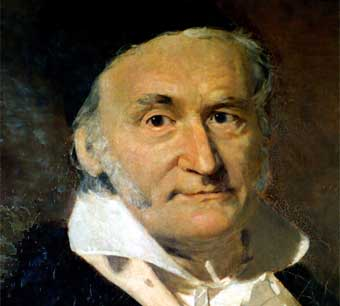
\includegraphics[width=4cm]{img-04/chap4.jpg}
	
	{\footnotesize \centering Carl F. Gauss (1777-1855) }}
{chap:complex}
  
\begin{blueshaded}
	L'home ha anat ampliant al llarg del temps la noció de nombre segons les seves necessitats. 
	
	Des de la prehistòria, els nombres naturals han servit per comptar. Els nombres enters negatius ens permeten resoldre equacions com $x+5=1$. De forma similar els nombres fraccionaris permeten resoldre $3x=2$. En l'antiga Grècia ja es sabia que no existia cap nombre racional que fos solució de $x^2=2$; D'aquí s'introduïren els nombres irracionals.
	
	El conjunt format pels nombres racionals i irracionals és el conjunt dels nombres reals. Aquests són tots els nombres amb els quals, de moment, hem treballat. 
	
%%	Existiran més tipus de nombres? Hi ha algun nombre que sigui la solució de l'equació $x^2+1=0$?
\end{blueshaded}   

\heading{Equacions de segon grau}
\begin{bluebox}
 \fontsize{10.5}{11}
  És possible trobar les solucions de l'equació $x^2-4x+13=0$?
  
  Si utilitzam la fórmula de les equacions de segon grau, trobam
  \[ x = \dfrac{4\pm \sqrt{4^2-4 \cdot 1\cdot 13}}{2} = \dfrac{4\pm \sqrt{-36}}{2} \]
  
  Donat que $\sqrt{-36}$ no és cap nombre real, deim que l'equació no té solucions reals. Però, separem  $\sqrt{-36}= \sqrt{36} \cdot \sqrt{-1} = 6 \sqrt{-1}$. Veim que el problema està en que no podem calcular $\sqrt{-1}$. 
  
  En 1777 Leonard Euler va anomenar $i=\sqrt{-1}$ com la unitat imaginària. D'aquesta forma podem escriure les solucions com:
   \[ x =  \dfrac{4\pm 6 i}{2}  = 2 \pm 3i\]
  Acabam d'escriure dos nombre complexos en forma binòmica.
\end{bluebox} 

\newpage
\section{Nombres complexos en forma binòmica}

	\begin{theorybox}
		\video[5]{164}{Introducció als nombres complexos}
			
		Es defineix la \textbf{unitat imaginària} $i$ com $i=\sqrt{-1}$. Es compleix que $i^2=-1$, $i^3=-i$, $i^4=1$, etc. \vspace{0.2cm}
		
		Els nombres de la forma $2i$, $5i$, $-\frac{3}{2}i$, $\cdots$ s'anomenen \textbf{imaginaris purs}.
 		
	 	 \begin{wrapfigure}{R}{0.2\textwidth}
	    	\vspace{-1cm} 
	    	\centering
	    	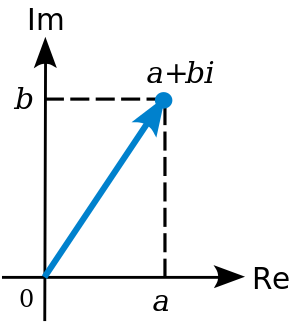
\includegraphics[width=0.19\textwidth]{img-04/pla-complex}
		 \end{wrapfigure}
 
			Un \textbf{nombre complex} en forma binòmica s'expressa com \linebreak $z=x+iy$, on $x$ s'anomena
			\textbf{part real} i $y$ la \textbf{part imaginària} del nombre.\vspace{0.2cm}
		 
				El nombres es representen sobre el \textbf{pla complex}. A l'eix horitzontal hi situam la part
			real i a l'eix vertical la part imaginària.  \vspace{0.2cm}
			
			El \textbf{complex conjugat} del nombre s'obté de canviar el signe de la part imaginària $z^* = x-iy$. El \textbf{mòdul} d'un nombre complex és la longitud 
			del nombre i s'obté de $|z|=\sqrt{x^2+y^2}$. Es compleix que $z\cdot z^*=|z|^2$.

			\vspace{0.5cm}
	\end{theorybox}

\begin{theorybox}[Operacions en forma binòmica]
	Suposau que es donen els nombres complexos $z_1 = 2-3i$ i $z_2 = 5+4i$. Amb aquests nombres podem fer les següents operacions:
	\begin{itemize}
		\item \textbf{Suma}:  \[ z_1 + z_2 = (2-3i) + (5+4i) = 7 + i\] 
		
		\item \textbf{Resta}: \[ z_1 - z_2 = (2-3i) - (5+4i) = -3 - 7i\]
		
		\item \textbf{Producte}:  \[ z_1 \cdot z_2 = (2-3i) \cdot (5+4i) = 10+8i-15i-12 \underset{\downarrow -1}{i^2} =22 -7i \]
		
		\item \textbf{Divisió}: \[ \frac{z_1} {z_2} = \frac{(2-3i)\cdot (5-4i)}{(5+4i)\cdot(5-4i)}=\frac{-2-23i}{41}\]
	\end{itemize}
\end{theorybox}
 
\begin{mylist}
\exer
Donats els següents nombres complexos:

\begin{center}
	$a=3i$, \quad
	$b=-2i$,\quad
	$c=5$,\quad
	$d=1+i$,\quad
	$p= -1 -i$
\end{center}

\begin{tasks}
	\task Representa'ls gràficament sobre el pla complex. Representa els seus conjugats.
	\task Representa gràficament les sumes: $a+b$, \quad $a+c$, \quad $b+d$, \quad $d+p$
	\task Representa gràficament els productes: $a\cdot i$, \quad  $b\cdot i$, \quad $c\cdot i$,\quad $d\cdot i$, \quad $p\cdot i$. Comprova que multiplicar per $i$ equival a girar el nombre complex 90º.
	%\task Calcula $Im(\frac{\bar z}{z})$ (\emph{Ajuda}: substitueix $z=x+i y$)
\end{tasks} 

\answers{Nombres i conjugats:\par 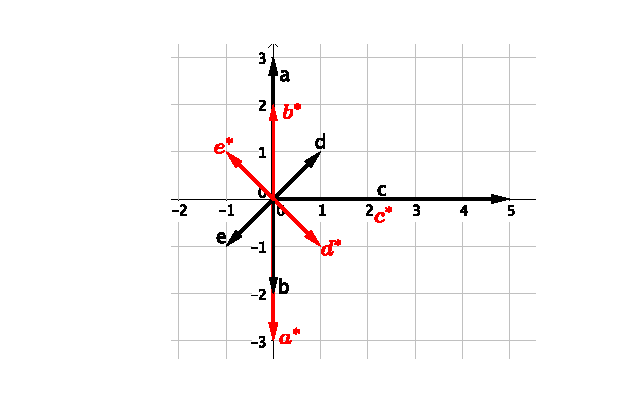
\includegraphics[width=0.44\textwidth]{img-sol/t4-1a}\par Operacions:\par 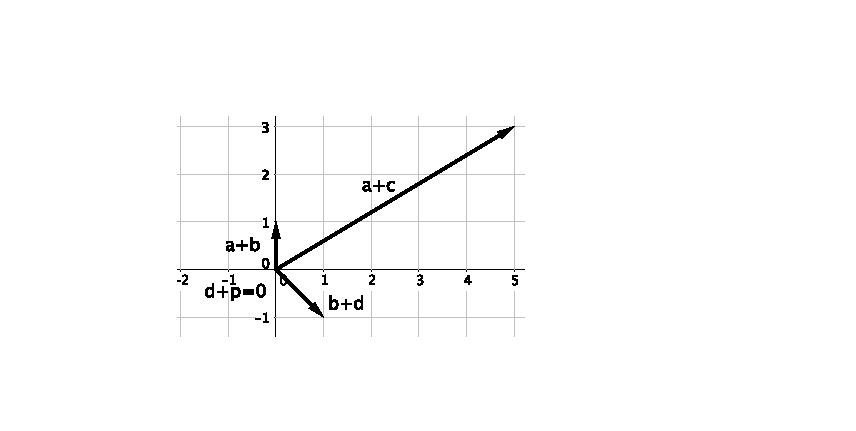
\includegraphics[width=0.44\textwidth]{img-sol/t4-1b}}
\vspace{3cm}

	\exer[1] Calcula

	\begin{tasks}(2)
		\task  $7 - 3i - (2 + 6 i)$
		\task  $(5 - 2i)\cdot (-3 i)$
		\task  $( 7 + 3 i) \cdot (-1 + 2 i)$
		\task  $(2+i)-i (1-2 i)$
		\task $(3-2 i) \cdot (3+ 2 i)$
		\task $(3 + 2i) - (1-i)\cdot(4-5i)$
	    \task $(1 + i)^2$
		\task $(1 - i)^4$
	\end{tasks}
	\answers[cols=2]{[
			 $5 -9i$,
			 $-6-15i$,
			 $-13+11i$,
			 0,
			 13,
			 $4 + 11i$,
			 $2i$,
			 $-4$]}
 ƒ
	\exer[1]
	Realitza les següents operacions amb nombres complexos:
	\begin{tasks}(2)
		\task $\dfrac{2-i}{1+3 i}$
		\task $\dfrac{5+10 i}{3-4 i}+\dfrac{2-i}{i}$
		\task $\dfrac{2+i}{4-3 i} + \dfrac{3+i}{5 i}$
		\task $\dfrac{68}{(1-i) \cdot (2-i) \cdot (3-i)}$
	\end{tasks}
\answers[cols=2]{[
		 $-{{1}\over{10}}-{{7\,i}\over{10}}$,
		 $-2$,
		 ${{2}\over{5}}-{{i}\over{5}}$,
		 ${{34\,i}\over{5}}$]}
	 
 
\end{mylist}

\begin{example}
	a) Per dividir dos nombres complexos, multiplicam i dividim pel complex conjugat del denominador.
	$\dfrac{2-i}{1+3 i} = \dfrac{(2-i)\cdot (1-3i)}{(1+3 i)\cdot (1-3i)} = \dfrac{2-6i-i-3}{10}=\dfrac{-1-7i}{10}$
	 
\end{example}


\begin{mylist}
	
	\exer Comprova les següents fórmules:
	\begin{tasks}(2)
		\task $(x+iy)^2=x^2-y^2+i2xy$
	%	\task $(x-iy)^2=x^2-y^2-i2xy$
		\task $(x+iy)\cdot (x-iy)=x^2+y^2=|z|^2$
	\end{tasks}
	

	
	\exer Calcula $a$ perquè el nombre complex $\dfrac{a+i}{3-i}$ tingui la seva part real igual a la seva part imaginària.
	\answers{Racionalitzant el nombre s'expressa com $\dfrac{3a-1}{10}+\dfrac{a+3}{10}i$. Si igualam les parts real i imaginària, això passa si $3a-1=a+3$, és a dir $a=2$}
\end{mylist}


\section{Nombres complexos en forma polar} 




\begin{theorybox}
		\video{165}{Operacions en forma polar}
	
	Un nombre complex $z=x+iy$ es pot expressar en forma polar donant el seu \textbf{mòdul} i l'angle que forma amb l'eix real.
	Aquest angle s'anomena \textbf{l'argument} del nombre complex. El nombre en \textbf{forma polar} s'expressa com $\mathbf{r_\theta}$ on
	\begin{equation*}
	r=\sqrt{x^2+y^2}, \,\,\,\,\, \,\,\,\,\,\,\,\,\,\, \theta = \arctg \dfrac{y}{x}
	\end{equation*}	
	Donat que hi ha infinits angles que tenen per tangent $y/x$, es defineix \textbf{l'argument principal} del nombre complex com un angle comprès entre $-\pi < \theta \leq \pi$ \; ($-180^\circ < \theta \leq 180^\circ$).
	
	De forma anàloga, es pot passar un nombre en forma polar a forma binòmica mitjançant
	\begin{equation*}
	z = r \cdot (\cos \theta + i \sin \theta)
	\end{equation*}	
	Aquesta forma també es coneix com \textbf{forma trigonomètrica}.
	

\end{theorybox}


\begin{mylist}
	\exer[1] Calcula el mòdul i l'argument principal dels següents nombres complexos:
	\begin{tasks}(4)
		\task  $\sqrt{3}-i$
		\task  $-2-2 i$
		\task  $1 - \sqrt{3} i $
		\task  $-4 i$
	\end{tasks}
	\answers[cols=1]{[
			 $|z|=2$;  $arg(z)=-30^\circ$,
			 $|z|=\sqrt{8}$;  $arg(z)=225 = - 135^\circ$,
			 $|z|=2$;  $arg(z)=-60^\circ$,
			 $|z|=4$;  $arg(z)=-90^\circ$]}
	
\end{mylist}
	
	\begin{example}
		a) 
		Donat $z=\sqrt{3}-i$, calculam el seu mòdul fent $|z|=\sqrt{(\sqrt 3)^2+(-1)^2}=\sqrt{4}=2$. L'argument el trobam de $\theta= \arctg(-1/\sqrt{3})=-30^\circ$.
		El nombre és $z=2_{-30^\circ}$
	\end{example}
 
 
 \begin{mylist}
 	
	\exer  
	Calcula el mòdul i l'argument principal dels següents nombres
 	complexos:

	\begin{tasks}(4)
		\task  $-3+3i$
		\task  $-3$
		\task $-3i$
		\task $3-3i$
	\end{tasks}
\answers[cols=1]{[$|z|=\sqrt{18}$;  $arg(z)=135^\circ$,
	$|z|=3$;  $arg(z)=180^\circ$,
	$|z|=3$;  $arg(z)=270^\circ$,
	$|z|=\sqrt{18}$;  $arg(z)=-45^\circ$]}


\exer Calcula l'argument principal dels següents nombres
complexos:

\begin{tasks}(3)
	\task  $\dfrac{-3}{\sqrt{3} + i}$
	\task  $\dfrac{-i}{1-i}$
	\task  $(1-i\sqrt{3})^7$
\end{tasks}
 \answers{[$z=\frac{3}{4}(-\sqrt{3}+i)$; $arg(z)=150^\circ$,
		  $z=\frac{1}{2}(1-i)$; $arg(z)=-45^\circ$,
		  $z=\left[2_{-60^\circ}\right]^7$; $arg(z)=-420^\circ=-60^\circ$]}
 
	\exer
	Expressa en forma polar els següents nombres complexos:

	\begin{tasks}(4)
		\task $i$ 
		\task $-i$
		\task $4 + 4i$ 
		\task $-4$
	\end{tasks}
\answers{[$1_{90^\circ}$, $1_{270^\circ}$, $4\sqrt{2}_{45^\circ}$, $4_{180^\circ}$]}

	
	\exer
	Expressa en forma polar els següents nombres complexos:

	\begin{tasks}(4)
		\task $5i$ 
		\task $-7i$
		\task $5 - 5i$ 
		\task $\sqrt{3}+i$

	\end{tasks}
\answers{[$5_{90^\circ}$, $7_{270^\circ}$, $5\sqrt{2}_{-45^\circ}$, $2_{30^\circ}$]}
	
	\exer[1] Expressa en forma binòmica els següents nombres complexos donats en forma polar:
	\begin{tasks}(2)
		\task De mòdul 2 i argument $\dfrac{\pi}{3}$
		\task De mòdul 3 i argument $-\dfrac{\pi}{4}$
		\task De mòdul 1 i argument $\dfrac{\pi}{2}$
		\task De mòdul 5 i argument $\dfrac{2 \pi}{3}$
	\end{tasks}
\answers[cols=1]{[ 
		 $2_{\,60^\circ}= 1 + \sqrt{3} i$, 
		 $3_{\,-45^\circ}= \frac{3\sqrt{2}}{2} - \frac{3\sqrt{2}}{2} i$, 
		 $1_{\,90^\circ}= i $, 
		 $5_{\,120^\circ}= -\frac{5}{2} + i \frac{5\sqrt{3}}{2}$]}
\end{mylist}
	
	\begin{theorybox}[Operacions en forma polar]
		L'avantatge de la forma polar és que les operacions es realitzen molt més ràpid.
		
		Si ens donen dos nombres en forma polar $r_\theta$ i $r'_{\theta'}$, 
		
		\textbf{Producte}: $r_\theta \cdot r'_{\theta'} = (r\cdot r')_{\theta+\theta'}$, multiplicam els mòduls i sumam els arguments.
		
		\textbf{Quocient}: $r_\theta : r'_{\theta'} = (r : r')_{\theta - \theta'}$, dividim els mòduls i restam els arguments.
		
		\textbf{Potència}:  $(r_\theta)^n = (r^n)_{n\cdot \theta}$, elevam el mòdul i multiplicam l'argument per l'exponent.
	\end{theorybox}
	
	\begin{resolt}[E]{Passa a forma polar, opera i comprova 
			
			$(1+i)^{16} = 2^8 = 256$.}
			En forma polar el nombre és $1+i=\sqrt{2}_{45^\circ}$. Per elevar el nombre a 16, elevam el mòdul i multiplicam l'argument per 16.
		
		\begin{equation*}
		(1+i)^{16}=(\sqrt{2}^{16} )_{16\cdot 45^\circ} = 2^8_{720^\circ}=2^8
		\end{equation*}
		
		On hem utilitzat que $720^\circ$ són dues voltes completes.
	\end{resolt}
	
\begin{mylist}	
 
	
	\exer
	Realitza les següents operacions amb nombres complexos, expressant-los

	prèviament en forma polar:

	\begin{tasks}(2)
		\task $\dfrac{\sqrt{2} i}{-2-2i}$
		\task $\left(\frac{1}{2} + \frac{\sqrt{3}i}{2}\right)^{30}$
	\end{tasks}


\answers[cols=1]{[$\dfrac{\sqrt{2} i}{-2-2i}=\dfrac{\sqrt{2}_{90}}{2\sqrt{2}_{-135}}=\dfrac{1}{2}_{225}=\dfrac{1}{2} (\cos 225 + i \sin 255)=-\dfrac{1}{4}(1+i)$, 
 $\left(\frac{1}{2} + \frac{\sqrt{3}i}{2}\right)^{30}=\left( 1_{60^\circ} \right)^{30}= 1_{1800^\circ}=1$
	]}
	
	\exer
	Realitza les següents operacions amb nombres complexos, expressant-los

	prèviament en forma polar:

	\begin{tasks}(3)
		\task $(\sqrt{3}+i)^{60}$
		\task $(4-4i)^{-11}$
		\task $\dfrac{(1-\sqrt{3} i)^{12}}{(-2-2i)^8}$
	\end{tasks}
	
	\answers[cols=1]{[$(\sqrt{3}+i)^{60}=(2_{30})^{60}=2^{60}_{1800}=2^{60}$,
		$(4-4i)^{-11}=(4\sqrt{2}_{-45^\circ})^{-11}=\frac{1}{2^{27}\sqrt{2}}_{495}=\frac{1}{2^{27}\sqrt{2}}_{135}=\frac{1}{2^{27}\sqrt{2}}(\cos 135 + i \sin 135)=\frac{1}{2^{28}} (-1+i)$,
		$\dfrac{(1-\sqrt{3} i)^{12}}{(-2-2i)^8}=\dfrac{(2_{-60^\circ})^{12}}{(2\sqrt{2}_{-135^\circ})^8}=
		\dfrac{2^{12}_{-720^\circ}}{2^{12}_{-1080^\circ}}=1_{360^\circ}=1$]}
	
\end{mylist}

\begin{theorybox}
 \textbf{Fórmula de Moivre: }
 \begin{equation*}
	(\cos \theta + i \sin \theta)^n = \cos(n \theta) + i \sin(n \theta)	 
 \end{equation*}
\end{theorybox}	
\vspace{-0.75cm}
\begin{example}
	Si utilitzam $n=2$ en la fórmula de Moivre:
	$	(\cos \theta + i \sin \theta)^2 = \cos(2 \theta) + i \sin(2 \theta) $
	
	Desenvolupam el quadrat del membre de l'esquerre:
		\[	\cos^2 \theta -  \sin^2 \theta + 2 i \sin \theta \cos \theta= \cos(2 \theta) + i \sin(2 \theta) \]
		
	Si igualam les part reals i imaginàries	trobam:
		\[ \begin{array}{l}	\cos (2\theta) = \cos^2 \theta -  \sin^2 \theta 	\\ \sin(2\theta) = 2\sin \theta \cos \theta  \end{array} \]
	que són les relacions de l'angle doble vistes en el tema \ref{chap:trig}.
\end{example}

	\begin{mylist}
		
	
	\exer Utilitza la fórmula de Moivre per expressar en funció de $\sin \theta$ i $\cos \theta$:
	\begin{tasks}(4)
		\task $\cos (-\theta)$
		\task $\sin (-\theta)$
		\task $\cos 3\theta$
		\task $\sin 3\theta$	
\end{tasks}
\answers[cols=1]{[$\cos (-\theta)=\cos \theta$, $\sin (-\theta)=-\sin\theta$, $\cos 3\theta=\cos^3 \theta - 3\sin^2 \theta \cos \theta$, $\sin 3\theta=3\sin \theta\cos^2 \theta - \sin^3\theta$]}

\end{mylist}

 
\section{Resolució d'equacions en el pla complex}
\begin{theorybox}
	\video{166}{Resolució d'equacions}
			Tot nombre complex té $n$ arrels enèsimes. Si ve expressat en forma polar $r_\theta$, les arrels són
	\begin{equation*}
		\sqrt[n]{r_\theta}= \left(\sqrt[n]{r}\right)_{\frac{\theta+k\cdot 360}{n}}
	\end{equation*}
	essent $k=0, 1, \cdots, n-1$.
	
	\vspace{0.5cm}

\end{theorybox}
	
\begin{mylist}

\exer Calcula les arrels i representa-les en el pla complex
\begin{tasks}(3)
	\task $\sqrt{-3 i}$
	\task $\sqrt{-9}$
	\task $\sqrt{1+\sqrt{3} \,i}$
	\task $\sqrt[3]{-27}$
	\task $\sqrt[3]{1-i}$
	\task $\sqrt[4]{-81}$
\end{tasks}

\answers{[$\sqrt{-3 i} \rightarrow$ $z=\pm\frac{\sqrt{6}}{2}(1-i)$ \par 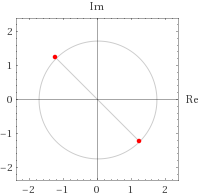
\includegraphics[width=0.3\textwidth]{img-sol/t4-15a}, 
	 $\sqrt{-9}\rightarrow$ $z=\pm 3i$ \par 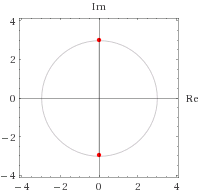
\includegraphics[width=0.3\textwidth]{img-sol/t4-15b}, 
	 $\sqrt{1+\sqrt{3} \,i}\rightarrow$ $z_1=\pm\frac{1}{2}(\sqrt{6}+i\sqrt{2})$ \par 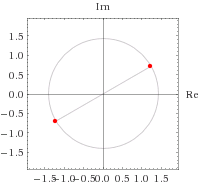
\includegraphics[width=0.3\textwidth]{img-sol/t4-15c},  
	 $\sqrt[3]{-27}\rightarrow$ $z_1=-3$; $z_2=\frac{3}{2}(1+i\sqrt{3})$; $z_3=\frac{3}{2}(1-i\sqrt{3})$ \par 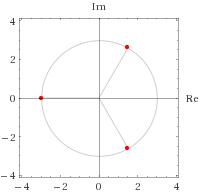
\includegraphics[width=0.3\textwidth]{img-sol/t4-15d}, 
	 $\sqrt[3]{1-i}\rightarrow$ $z_1\approx 1.084-0.29i$; $z_2 \approx -0.29 +1.084i$; $z_3=-0.794-0.794i$ \par 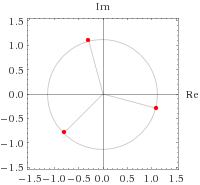
\includegraphics[width=0.3\textwidth]{img-sol/t4-15e}, 
	 $\sqrt[4]{-81}\rightarrow$ $z=\pm \frac{3\sqrt{2}}{2}(1+i)$; $z=\pm \frac{3\sqrt{2}}{2}(1-i)$\par 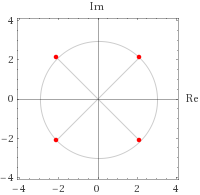
\includegraphics[width=0.3\textwidth]{img-sol/t4-15f}]}
\end{mylist}

\begin{example}
	a) Primer expressam el nombre $z=-3i$ en forma polar. Sabem que té mòdul 3 i argument 270º. Tenim dos possibles resultats de l'arrel quadrada
	\begin{equation*}
		\sqrt{3_{270^\circ}} = \left\{ 
		\begin{array}{l}
			\sqrt{3}_{270/2} = \sqrt{3}_{135^\circ} \\
			\sqrt{3}_{(270+360)/2} = \sqrt{3}_{315^\circ}
		\end{array}
		 \right.
	\end{equation*}
\end{example}


\begin{mylist}
	

\exer Calcula les arrels cinquenes de la unitat i representa-les en el pla complex. Calcula també totes les arrels cinquenes de $-1$ i representa-les.

\answers[cols=1]{[$\sqrt[5]{1} \rightarrow$ $z= 1$; $z \approx 0.309 \pm 0.9511i$; $z\approx -0.809\pm 0.5878 i$ \par 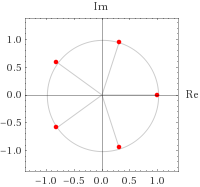
\includegraphics[width=0.3\textwidth]{img-sol/t4-16a},
	$\sqrt[5]{-1} \rightarrow$ $z=-1 $; $z \approx 0.809\pm 0.588 i$; $z=-0.309 \pm 0.9511 i$ \par 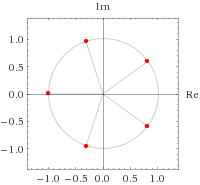
\includegraphics[width=0.3\textwidth]{img-sol/t4-16b}]}

	\exer Resol les equacions:
\begin{tasks}(4)
	\task $x^3=-27$
	\task $x^4=-81$
	\task $x^5+32=0$
	\task $x^3-8=0$
\end{tasks}

\answers[cols=1]{[$x=\sqrt[3]{-27}$ exemple, $x=\sqrt[4]{-81}$ exercici anterior f), $x=\sqrt[5]{-32}\rightarrow$ $z=-2$; $z\approx 1.618 \pm 1.1756 i$; $z=-0.618 \pm 1.9021 i$; \par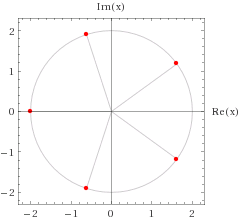
\includegraphics[width=0.3\textwidth]{img-sol/t4-17c}, $x=\sqrt[3]{8}\rightarrow$ $z=2$; $z=-1\pm \sqrt{3}i$;\par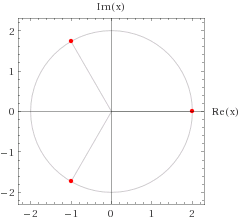
\includegraphics[width=0.3\textwidth]{img-sol/t4-17d} ]}

\end{mylist}

\begin{example}
	a) $x^3=-27$ implica que $x=\sqrt[3]{-27}$ que evidentment té una solució real $x=-3$. Per trobar les altres dues arrels expressam el nombre en forma polar $-27=27_{180^\circ}$ i 
	en feim l'arrel cúbica.
	
	\begin{minipage}{0.7\textwidth}

	\begin{equation*}
	\sqrt[3]{27_{180^\circ}} = \left\{ 
	\begin{array}{l}
	3_{180/3} = 3_{60^\circ} \\
	3_{(180+360)/3} = 3_{180^\circ} \\
	3_{(180+2\cdot 360)/3} = 3_{300^\circ}  
	\end{array}
	\right.
	\end{equation*}
	
Si finalment passam les tres arrels a forma binòmica trobam \linebreak $x=-3$, $x=3(\frac{1}{2}+\frac{\sqrt{3}}{2}i)$, $x=3(\frac{1}{2}-\frac{\sqrt{3}}{2}i)$. Si representam aquests tres nombres sobre el pla
complex veim que formen els vèrtexs d'un triangle equilàter.
	\end{minipage}
	\begin{minipage}{0.3\textwidth}
		\begin{center}
		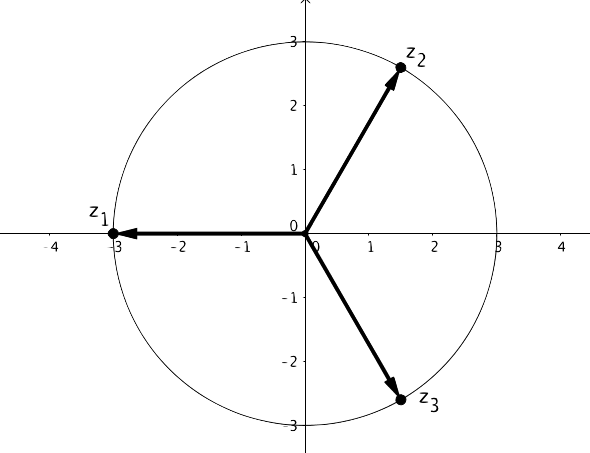
\includegraphics[width=0.95\textwidth]{img-04/chap-complex-3root}		
		\end{center}
	\end{minipage}

	 
\end{example}

\begin{mylist}

	\exer
	Resol les equacions, obtenint les arrels reals i complexes:

	\begin{tasks}(3)
		\task $x^2=-1$
		\task $x^3=-8$
		\task $x^4+16=0$
	\end{tasks}

\answers[cols=1]{[$x^2=-1\rightarrow$ $z=\pm i$, $x^3=-8 \rightarrow$ $z=-2$; $z=1+\sqrt{3}i$; $z=1-\sqrt{3}i$, $x^4+16=0 \rightarrow$ $z=\pm 2$; $z=\pm 2i$]}
 
	\exer
	Calcula les arrels enèsimes de la unitat, per a $n$ = 2, 3 i 4.
	Representar-les gràficament, i comprova que estan sobre la
	circumferència de radi 1, i són els vèrtexs d'un polígon regular.
	
\answers[cols=1]{[$\sqrt{1} \rightarrow$ $z=\pm 1$, $\sqrt[3]{1} \rightarrow$ $z=1$; $z=\frac{1}{2}(-1\pm \sqrt{3})$ \par 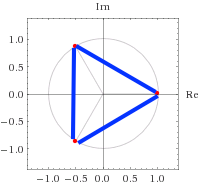
\includegraphics[width=0.3\textwidth]{img-sol/t4-19b}, $\sqrt{4} \rightarrow$ $z=\pm 1$; $z=\pm i$ \par 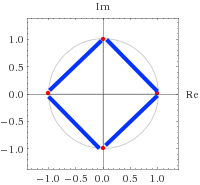
\includegraphics[width=0.3\textwidth]{img-sol/t4-19c}]}

\exer Resol l'equació $z^2+3z-1=0$.
\answers{Dues arrels reals: $z=\dfrac{-3\pm \sqrt{13}}{2}$}

	 
\exer Calcula tots els nombres complexos $z$ pels quals:
	\begin{tasks}(2)
		\task $z^6+64=0$
		\task $(z^2+3z-2)^2 - (2z^2-z+1)^2 =0$
		\task $z^6+z^5+z^4+z^3+z^2+z+1=0$
	\end{tasks}

\answers[cols=1]{[$z=\sqrt[6]{-64}$; $z=\pm 2i$; $z=\pm(\sqrt{3}+i)$; $z=\pm(\sqrt{3}-i)$, $-3z^4+10z^3-10z+3=-(z-3)(z-1)(z+1)(3z-1)$ té solucions reals $z=3$; $z=\pm 1$; $z=1/3$, Identificam una progressió geomètrica de raó $z$: La seva suma\par $\dfrac{z^7-1}{z-1}=0$ implica que $z^7=1$; són les arrels setenes de 1 (1 no serveix): Totes les arrels són per tant complexes: $z=-0.9 \pm 0.434 i$; $z=-0.22\pm 0.975 i$; $z=0.623 \pm 0.782$]}

\exer Resol aquestes equacions en el pla complex. Representa les solucions gràficament.
\begin{tasks}(2)
	\task $z^2+4i=0$
	\task $z^3+8i=0$ 
	\task $iz^3-27=0$
	\task $iz^4+4=0$
\end{tasks}

\answers{[Veure exemple;\par 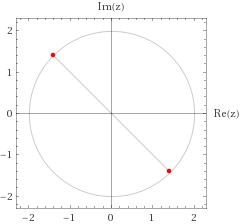
\includegraphics[width=0.3\textwidth]{img-sol/t4-22a}, $z=2i$; $z=-\sqrt{3}-i$; $z=\sqrt{3}-i$;\par 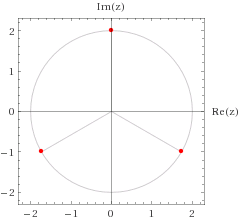
\includegraphics[width=0.3\textwidth]{img-sol/t4-22b}, 
	$z=3i$; $z=-\frac{3}{2}(\sqrt{3}+i)$;  $z=\frac{3}{2}(\sqrt{3}-i)$;\par 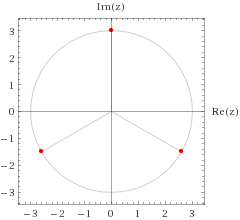
\includegraphics[width=0.3\textwidth]{img-sol/t4-22c}, 
	$z=\pm (1.3066+0.5412 i)$; $z=\pm (0.5412-1.3055 i)$;\par 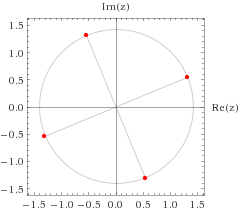
\includegraphics[width=0.3\textwidth]{img-sol/t4-22d} ]}

\end{mylist}

\begin{example}[*]
	a)  $z^2+4i=0$
	
	Començant aïllant la incògnita $z=\sqrt{-4i}$. Tot seguit hem de calcular totes les arrels (complexes) del nombre $-4i$. Per això, l'expressam en forma polar $-4i=4_{270^\circ}$.
	
	\[ \sqrt{4_{270^\circ}} = \left\{
		\begin{array}{l}
		\sqrt{4}_{\frac{270^\circ}{2}} = 2_{135^\circ} \\ 
		\sqrt{4}_{\frac{270^\circ+360^\circ}{2}} = 2_{315^\circ}
		\end{array} 
		\right.  \]
		
	Finalment, podem expressar les dues arrels en forma binòmica:
	
	\[ \left\{
	\begin{array}{l}
  2_{135^\circ} = 2 (\cos 135 + i\sin 135)= -\sqrt{2}+i\sqrt{2} \\ 
  2_{315^\circ} =  2 (\cos 315 + i\sin 315)= \sqrt{2}-i\sqrt{2}
	\end{array} 
	\right. \]
	
\end{example}

\begin{mylist}
 
\exer Calcula les quatre arrels de $z^4+9=0$ i utilitza-les per factoritzar $z^4+9$ amb dos polinomis de segon grau amb coeficients reals.
\end{mylist}


%%%%%%%%%%%%%%%%%%%%%%%%%%%%%%%%%%%%%%%%%%%%%%%%%%%%%%%%%%%
%%%%%%%%%%%%%% AUTOAVALUACIO
%%%%%%%%%%%%%%%%%%%%%%%%%%%%%%%%%%%%%%%%%%%%%%%%%%%%%%%%%%%

\begin{autoaval}{40}

\begin{mylist}
	
	\vspace{-2cm}
		
	\exer[2]  \begin{minipage}[t]{0.6\textwidth}
		Donats els nombres complexos de la figura es demana calcular:
		\begin{tasks}
			\task $z_1^* - z_3$
			\task $z_1^2$
			\task $|z_3|(z_1+z_2)$
			\task $\dfrac{z_1}{z_2}$
		\end{tasks}	
	\end{minipage}
	\begin{minipage}{0.4\textwidth}
		\centering
		\vspace{2.5cm}
		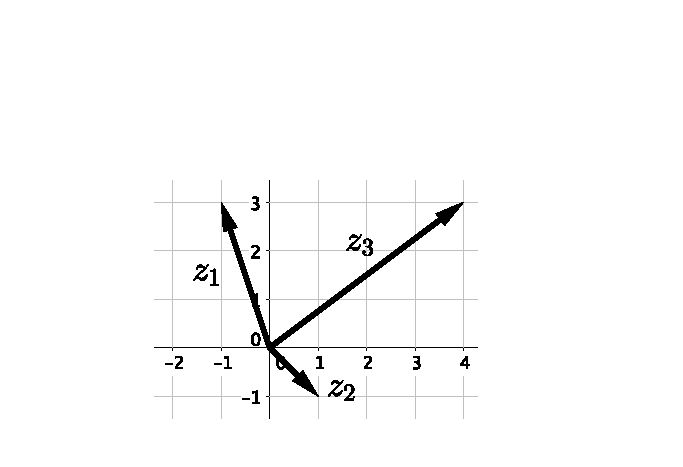
\includegraphics[width=0.7\textwidth]{img-04/autoaval-complexos1}
	\end{minipage}
\answers[cols=2]{[$-5-6i$, $-8-6i$, $10i$, $-2+i$]}

	
\exer[2]  Calcula
$\dfrac{(3+2 i)\cdot(3-2i)}{(2+3i)^3}$
\answers{$-46+63i$}

\exer[2] Resol l'equació: $z^2 - 10z+29=0$
\answers{$z_1=5+2i$, $z_2=5-2i$}

\exer[2] Donada l'expressió $\dfrac{1-i}{2-k i}$, troba els valors de $k$ pels quals l'expressió és: 
\begin{tasks}
	\task Real
	\task Imaginari pur.
\end{tasks}
\answers{[Real $k=-2$, Imaginari pur $k=-2$]}

\exer[2] Calcula el valor que ha de prendre $x$ per què el mòdul de $\dfrac{x+2i}{1-i}$ sigui igual a 2.
\answers{$x=\pm 2$}

\exer[2] Calcula el mòdul i l'argument principal del següent nombre
complex $-3 + 3i$:
\answers{$3\sqrt{2}$, $3\pi/4$}

\exer[2] Expressa en forma binòmica el nombre complex de
mòdul 2 i argument $\pi/3$
 
\answers{$1+\sqrt{3}i$}

\exer[2] Calcula $(1 + i)^6$ passant prèviament a forma polar.
 
\answers{$-8i$}

\exer[2] Expressa en forma trigonomètrica el següent nombre complex
$5i$.
\answers{$5(\cos(\pi/2) +i \sin(\pi/2)$}



\exer[2] Calcula les arrels cúbiques de $4\sqrt{3}-4i$. Representa-les gràficament.
\answers{$z_1=2_{110^\circ}$, $z_2=2_{230^\circ}$, $z_3=2_{350^\circ}$}

\end{mylist}
\end{autoaval}

\newpage
\resum
\begin{center}
\setlength\LTleft{0pt}
\setlength\LTright{0pt}
\ftimes{10.5}{11}
\renewcommand{\arraystretch}{1.5}
\fontsize{10.5}{11}
\begin{longtable}[h]{|>{\raggedleft\arraybackslash}p{0.2\textwidth}|p{0.8\textwidth}|}
	\toprule %inserts double horizontal lines
	\rowcolor{lightgray}
	
	\textbf{Apartat} & \textbf{Resum} \\   [0.5ex] 
	\toprule  \hline
	
	\cellcolor{lightgray}\noindent \textbf{Unitat imaginària} & $i^2=-1$ $\leftrightarrow$ $i=\sqrt{-1}$    \\ [0.5ex]\hline
	
	\cellcolor{lightgray}\noindent \textbf{Nombre en forma binòmica}  & $z=x+iy$ 
	
	 \sample{
	 $z=2+3i$, té part real 2 i part imaginària 3 
	 }
	  \hline
	
	\cellcolor{lightgray}\noindent \textbf{Complex conjugat} & $z^*=x-iy$ 
	
	 \sample{$\bar z = 2 - 3 i$} \hline
	
	\cellcolor{lightgray}\noindent \textbf{Suma de complexos} & $(x+iy)+(o+iv)=(x+o)+i(y+v)$ 
	
	 \sample{ $(2+3i)+(4+5i)=6+8i$ } \hline
	
	\cellcolor{lightgray}\noindent \textbf{Producte de complexos} & $(x+iy)\cdot(o+iv)=(x\cdot o - y\cdot v)+i(x\cdot v+ y \cdot o)$ 
	
	 \sample{ $(2+3i)\cdot(4+5i)=2+4i-i-2i^2=4+3i$ } \hline
	
	\cellcolor{lightgray}\noindent \textbf{Divisió de complexos} & Es multiplica numerador i denominador pel complex conjugat del denominador. Així s'aconsegueix un denominador real. 
	
	\sample{
	 $\frac{2}{1+i} = \frac{2\cdot(1-i)}{(1+i)\cdot(1-i)}=\frac{2\cdot(1-i)}{2}=1-i$  } \hline		
	
	\cellcolor{lightgray}\noindent \textbf{Forma polar} & $r_\theta$ amb $r=\sqrt{x^2+y^2}$ i $\theta=\arctg\frac{y}{x}$ 
	
	\sample{
	 $ z = 2 + 3 i$, $r=\sqrt{13}$, $\theta=\arctg \frac{3}{2}$  } \hline
	
	\cellcolor{lightgray}\noindent \textbf{Forma trigonomètrica} & $z=r\cdot(\cos\theta + i \sin \theta)$   
	
	\sample{
	 Si tenim $z=2_{30^\circ}$,  $z=2\cdot(\cos 30^\circ + i\sin 30^\circ)$  }\hline
		
	\cellcolor{lightgray}\noindent \textbf{Producte en forma polar} & $z=r_\theta$ i $z'=r'_\alpha$, aleshores $z\cdot z'= (r\cdot r')_{\theta+\alpha}$. Multiplicam els mòduls i sumam els arguments.   
	
	\sample{ Si tenim $z=2_{30^\circ}$ i $z'=3_{50^\circ}$,   $z\cdot z'=(2\cdot 3)_{30+50^\circ}=6_{80^\circ}$  } \hline
		
	\cellcolor{lightgray}\noindent \textbf{Divisió en forma polar} & $z=r_\theta$ i $z'=r'_\alpha$, aleshores $z / z'= (r / r')_{\theta-\alpha}$. Dividim els mòduls i restam els arguments.
	   
	\sample{ Si tenim $z=2_{30^\circ}$ i $z'=3_{50^\circ}$,   $z / z'=(2 / 3)_{30-50^\circ}=(2/3)_{340^\circ}$  } \hline	
	
	\cellcolor{lightgray}\noindent \textbf{Potència en forma polar} & $z=r_\theta$, aleshores $z^n= (r^n)_{n\cdot\theta}$. Elevam el mòdul i multiplicam l'argument per $n$.   
	
	 \sample{ Si tenim $z=2_{30^\circ}$ i volem calcular  $z^3= (2 ^ 3)_{3\cdot 30^\circ}=8_{90^\circ}$  } \hline	
		
	\hline \bottomrule
\end{longtable}
\end{center}
  